\documentclass[notoc]{porocilo}
\usepackage{tikz}
\usetikzlibrary{positioning, shapes.geometric}

\input{.local/mafijski_praktikum}
\projecttitle{Strojno učenje za kategorizacijo podatkov}
\instructions{Na spletni učilnici je na voljo material (koda, vzorci) za ločevanje dogodkov Higgsovega bozona
    od ostalih procesov ozadja. V naboru simuliranih dogodkov je 18 karakteristik (zveznih kinematičnih
    lastnosti), katerih vsaka posamezno zelo slabo loči `signal' od ozadja, z uporabo BDT ali (D) \!NN,
    pa lahko tu dosežemo zelo dober uspeh. Na predavanjih smo si ogledali glavne aspekte pomembne
    pri implementaciji ML, kot so uporaba ustreznih spremenljivk (GIGO), učenje in prekomerno učenje
    (training/overtraining), vrednotenje uspeha metode kot razmerje med učinkovitostjo (efficiency) in
    čistostjo (precision) vzorca (Receiver Operating Characteristic, ROC). Določi uspešnost obeh metod
    (in nariši ROC) za nekaj tipičih konfiguracij BDT in DNN, pri čemer:
    \begin{itemize}
        \item študiraj vpliv uporabljenih vhodnih spremenljivk --- kaj, če vzamemo le nekatere?
        \item študiraj BDT in NN in vrednoti uspešnost različnih nastavitev, če spreminjaš nekaj konfiguracijskih parametrov (npr. število perceptronov in plasti nevronskih mrež pri DNN in število dreves pri BDT).
    \end{itemize}
}

\begin{document}
\selectlanguage{slovene}
\maketitle
\section{Uvod}
Nobelova nagrada iz fizike podeljena leta 2024 je le še dodatno potrdila močno povezavo med strojnim učenjem in fiziko. Ob večanju količine podatkov ustvarjenih ob modernih eksperimentih je uporaba takšnih metod ključna za uspešno obdelavo rezultatov. Arhetipski primer takšnega poskusa, ki se je globoko vrezal v zgodovino je tudi detekcija Higgsovega bozona iz leta 2012 v Cernu. V tej nalogi se bomo lotili zaznave delca iz javno dostopnih podatkov podobnega poskusa. Za obdelavo pa bomo uporabili strojno učenje.

\section{Nabor podatkov}
Pri nalogi bomo uporabljali znan nabor podatkov pri zaznavi Higgsovega bozona~\cite{Higgs2014}. Celoten set vključuje 11M podatkov, od katerih pa bomo zaradi omejitev mojega računalnika uporabljali le 500k. Dimenzionalnost podatkov pa bomo iz originalnih 28 dimenzij zbili na 18. Med temi so kinematične lastnosti Leptona in štirih nastalih curkov, za katere vemo tudi o prisotnosti b kvarka. Poznamo tudi smer in velikost manjkajoče energije, zaradi delcev, ki so brez interakcije kot so nevtrini. Preostale spremenljivke so invariantne mase. Izmed teh možnih lastnosti pri tej analizi ne uporabimo štirih lastnosti o prisotnosti b kvarka v vsakem izmed curkov in šestih smeri energije, torej za štiri curke, manjkajočo energijo in lepton. S takšnim izborom dobimo iskanih 18 latnosti na podlagi katerih podatke nato klasificiramo v dva razreda. Z $0$ ali \textit{ozadje} označimo dogodke, ki niso proizvedli Higgsovega bozona in z $1$ ali \textit{signal} tiste, ki so. Tako naš problem postane binarna klasifikacija. Med podatki je delež signala $0,529$. Pred samo obdelavo podatke še reskaliramo, tako da postavimo najmanjšo vrednost lastnosti na 0 in največjo na 1.

\insertfig[0.85]{feat1.pdf}{Porazdelitve signala in ozadja po napovednih spremenljivkah. Prvi del.}{feat1}
\insertfig[0.85]{feat2.pdf}{Porazdelitve signala in ozadja po napovednih spremenljivkah. Drugi del.}{feat2}

Da bomo iz napovednih spremenljivk lahko sploh klasificirali dogodke, se morata razreda dovolj razlikovati po njih. Porazdelitve si lahko pogledamo na slikah~\ref{fig:feat1} in~\ref{fig:feat2}. Zaradi rahlega, vendar prisotnega, neravnovesja med razredoma seveda uporabimo normirane porazdelitve. Iz samih slik in očesnega testa bi ocenil za najbolj ključne \texttt{m\_bb}, \texttt{m\_wbb} in \texttt{m\_wwbb}. Medtem ko \texttt{m\_jj} izgleda enaka za oba razreda. Med podatki lahko pogledamo še za medsebojno korelacije med napovednimi spremenljivkami, slika~\ref{fig:corr}. Opazimo predvsem močno povezanost med določenimi invariantnimi masami in majhno negativno korelacijo med manjkajočo energijo in prečno gibalno količino leptona, kar zveni fizikalno smiselno povezano z ohranitvijo energije. Zanimiv je tudi vzorec šahovnice, ki kaže na dodatno povezanost med enakimi tipi podatkov, torej tistih, ki govorijo o magnitudi in tistih, ki govorijo o smeri v kinematiki.

% \insertfig[0.8]{corr.pdf}{Korelacijska matrika med napovednimi spremenljivkami.}{corr}

% \insertfig[0.8]{lda.pdf}{Ločitev podatkov z LDA.}{lda}

\begin{figure}
    \centering
    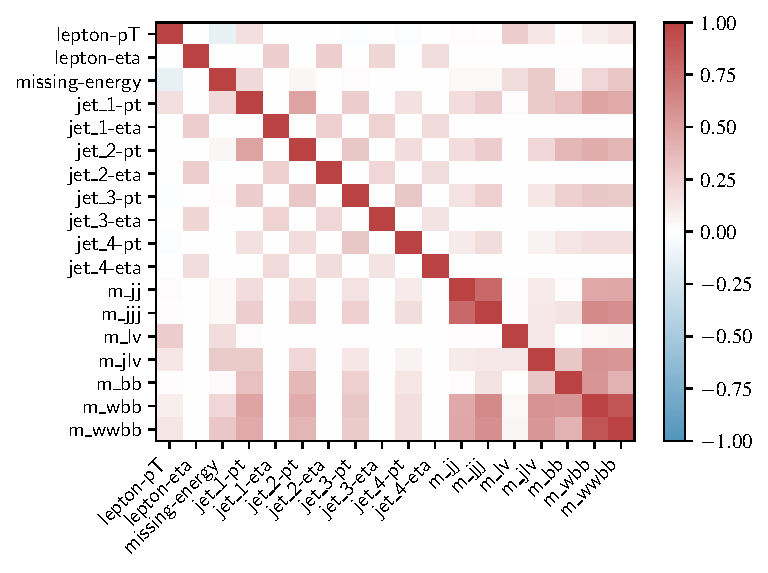
\includegraphics[width=0.85\textwidth]{corr.pdf}
    \caption{\label{fig:corr} Korelacijska matrika med napovednimi spremenljivkami.}

    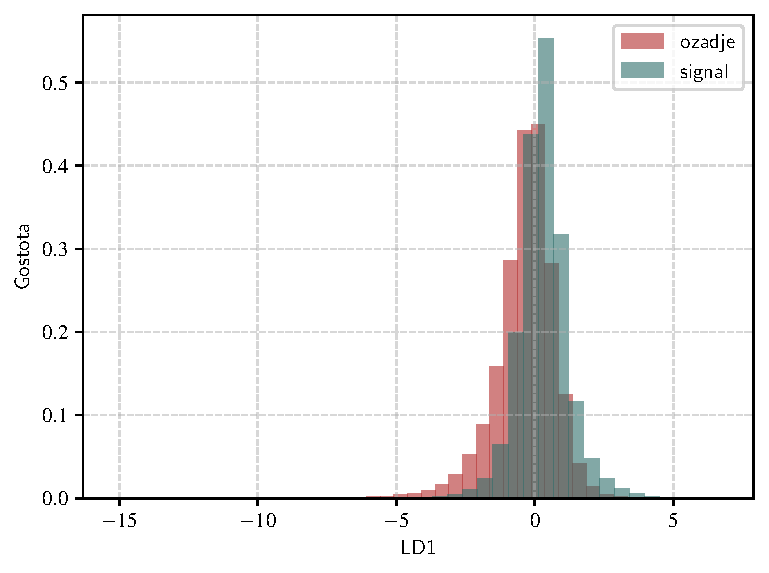
\includegraphics[width=0.75\textwidth]{lda.pdf}
    \caption{\label{fig:lda} Ločitev podatkov z LDA.}
\end{figure}

\section{Linearna diskriminantna analiza}
Iz slik~\ref{fig:feat1} in~\ref{fig:feat2} smo z oceno na oko poskusili ugotoviti katere spremenljivke najbolje ločijo med razredoma, vendar pa lahko tudi to storimo bolje, in sicer z linearno diskriminantno analizo. Le ta nam, zaradi binarne narave problema, podatke postavi na premico. Povemo lahko tudi katere napovedne spremenljivke najbolje ločijo razreda med seboj. Ločitev vidimo na sliki~\ref{fig:lda}. Iz te slike izgledata razreda precej slabo ločena. Vendar lahko tudi to ocenimo kvantitativno, in sicer z ROC krivuljo in površino pod le to, torej AUC metriko. Rezultat vidimo na sliki~\ref{fig:roc_lda}, kjer je vrednost AUC $0,683$. Za najpomembnejše diskriminatorje pa so se izkazale tri invariantne mase, katere smo pričakovali. Najslabši pa je \texttt{jet\_3-eta} in ne \texttt{m\_jj}. Skupno se ocena na oko ni močno razlikovala od kvantitativnih rezultatov.

\insertfig[0.8]{roc_lda.pdf}{ROC krivulja za LDA klasifikator.}{roc_lda}

\section{Odločitvena drevesa}
Linearna diskriminantna analiza iz prejšnjega poglavja je že ena izmed klasičnih metod strojnega učenja. V tem poglavju pa bomo prešli na odločitvena drevesa. Za izhodiščni model si izberemo LDA in metriko AUC, po kateri doseže vrednost $0,683$. Cilj preostalih modelov je torej preseči to vrednost. Odločitveno drevo je značilen primer strojnega učenja, kjer se na vsakem koraku odločamo, kako določen parameter omejiti in na podlagi tega narisati mejo med razredoma. Model je zelo interpretabilen in enostaven, vendar pa se pogosto že z le malo izboljšavami kosa z najbolj naprednimi metodami v strojnem učenju.

Najprej si poglejmo preprosto posamezno odločitveno drevo. Tukaj z AUC metriko dobimo vrednost $0,741$, kar premaga LDA. Vemo pa, da lahko z združevanjem modelov v ansamble izboljšamo njihovo napovedno moč. Pogoj je le, da je posamezen model boljši kot met kovanca, torej boljši kot $0,5$, kar v našem primeru odločitveno drevo je. Uporabili bomo Catboost, ki je sestavljen iz odločitvenih dreves, med seboj pa jih združuje preko gradienta. Vsako naslednje drevo torej pogleda napake trenutnega modela in jih popravi, za fizika zveni ideja zelo podobna perturbaciji. Za naš primer si izberemo mejo 1000 dreves, ki jih nato združimo na opisani način in dobimo nov ansambelski model, ki pa doseže AUC vrednosti $0,819$, kar je še en velik korak naprej v primerjavi z že obravnavanima modeloma.

\section{Nevronske mreže}
Reševanje problema se lahko lotimo tudi z nevronskimi mrežami, kar je nekoliko bolj moderen pristop. Izbrali bomo usmerjeno nevronsko mrežo z 18 vhodnimi nevroni, zaradi 18 dimenzij vhodnih parametrov, temu sledita 2 skriti plasti s po 50 nevroni, na koncu pa še z enim izhodnim nevronom, ki ima sigmoid aktivacijsko funkcijo, kar povzroči, da je izhod med 0 in 1. Nato na podlagi postavitve meje med razredoma dobimo ROC krivuljo in iz tega AUC metriko. Preostale plasti uporabljajo ReLu aktivacijsko funkcijo. Podatke razdelimo na trening, test in validacijsko podmnožico v razmerju $18:2:5$. Za funkcijo izgube uporabimo prečno entropijo, za optimizatorja pa Adam. Model smo nato trenirali 50 epoh in dobili končno vrednost AUC metrike na neodvisnih validacijskih podatkih enako $0,814$, kar je precej bolje kot LDA. Tak model ima skupno količino parametrov, ki jih lahko treniramo $3551$. Poglejmo pa si sedaj še nekoliko bolj napreden model, kjer vsaki skriti plasti dodamo še opuščanje nevronov s stopnjo opuščanja $0,2$. Poleg tega sedaj modelu dodamo upravljalnik učne stopnje, ki v primeru stagnacije padanja izgube zmanjša stopnjo učenja, in zgodnje končanje treniranja prav tako po daljši stagnaciji. Ta torej nekoliko kompleksnejši model ima učljivih parametrov še vedno enako in po 88 epohah doseže AUC vrednost $0,815$, kar je približno enako enostavnejši mreži. Nazadnje poskusimo še z večjo nevronsko mrežo, in sicer sedaj vzamemo enostavnejšo mrežo in dodamo še tretjo skrito plast s 50 nevroni. Taka sprememba poveča skupno število učnih parametrov na $6101$, zanima pa nas predvsem ali smo z velikostjo modela bližje prekomernega ali premalega prileganja. AUC vrednost za tak model po $100$ epohah treninga je $0,821$.

\section{Primerjava modelov}
Zaznavo Higgsovega bozona, ki smo jo uspeli spraviti v binarno klasifikacijo smo reševali na šest različnih načinov. Vsi uporabljeni modeli in njihove AUC vrednosti so zapisane v tabeli~\ref{tab:models}. Vidimo, da je LDA, ki smo ga vzeli za izhodiščni model precej slabši od ostalih, torej smo dosegli cilj, da ga premagamo. Izmed naprednejših pa ima najboljši rezultat večja izmed nevronskih mrež, vendar sta tudi obe manjši nevronski mreži in Catboost zelo blizu. Čeprav nisem eksplicitno meril, sem pri poganjanju modelov opazil precejšnjo razliko v času, in sicer je izmed boljših štirih metod Catboost precej hitrejša za trening od ostalih, kar je lahko razlog za preferenco pred nevronskimi mrežami, ki pa so navadno bolj uporabne za bolj kompleksne probleme.

\begin{table}
    \centering
    \caption{\label{tab:models} Tabela uporabljenih modelov in njihove AUC vrednosti.}
    \begin{tabular}{l c c c}
        Model                           & AUC     \\
        \hline
        Linearna diskriminantna analiza & $0,683$ \\
        Odločitveno drevo               & $0,741$ \\
        Catboost                        & $0,819$ \\
        Enostavna Nevronska mreža       & $0,814$ \\
        Naprednejša Nevronska mreža     & $0,815$ \\
        Večja Nevronska mreža           & $0,821$
    \end{tabular}
\end{table}

\section{Zaključek}
Pri nalogi smo torej uporabljali različne metode strojnega učenja za reševanje problema binarne klasifikacije dogodkov, kjer zaznamo Higgsov bozon in tistih, kjer ga ne. Preizkusili smo 5 modelov, in sicer LDA, odločitveno drevo, Catboost in nevronski mreži. Modele smo ocenjevali z AUC metriko. Izmed izbranih primerov se je najbolje izkazala večja izmed nevronskih mrež, manjši dve in Catboost pa so bili zelo blizu. Očitne omejitve uporabljenih metod so relativno malo število podatkov proti velikosti celotnega seta podatkov, prav tako sem omejen iz strani računske moči in menim, da bi z večjimi modeli rezultati prav tako bili boljši, na kar kaže dejstvo, da je najbolje deloval največji model. Prav tako je strojno učenje zelo obsežno področje, katerega sem se v tej nalogi komaj dotaknil. Na podatkih bi lahko uporabili še PCA metode, naključne gozdove, v nevronske mreže bi lahko dodali dodatne residualne povezave, lahko bi uporabili transformer arhitekturo, in še mnogo, mnogo drugih metod.

S tem poročilom zaključujem mafijski praktikum. Pri pregledu poročil od začetka do konca vidim velik napredek. Naučil sem se bolje uporabljati \LaTeX in upodabljati podatke na različne načine. Prav tako sem spoznal precej numeričnih metod iz praktične perspektive.

Nazadnje še seveda časovna statistika, za to poročilo sem skupaj porabil nekje $\SI{12}{\hour}$, od česar jih je precej šlo za tehnične stvari, kot so ukvarjanje s prenosom podatkov, posodabljanjem knjižnic in poskušanjem uporabe Google Colab, kar žal ni uspelo, saj sem prehitro porabil brezplačne kredite na GPU pospeševalnikih. Ker pa je to zadnje poročilo zaključujem še s podatkov, da sem za vsa poročila porabil nekje $\SI{116}{\hour}$ in še precej ob pogovoru o nalogah s sošolci.

\begin{thebibliography}{9}
    \bibitem{Higgs2014}
    P. Baldi, P. Sadowski, and D. Whiteson,
    ``HIGGS Data Set'',
    UCI Machine Learning Repository,
    University of California, Irvine, School of Information and Computer Sciences,
    2014.
    \url{https://archive.ics.uci.edu/dataset/280/higgs}
\end{thebibliography}
\end{document}

